\begin{frame}
  \frametitle{Time-Dependent Simulations with the Hybrid Method}
%  I investigated two transient scenarios based on actual MSRE experiments:
  Time-dependent reactivity-initiated simulation based on an MSRE rod drop experiment.
  \begin{block}{\textbf{MSRE Rod Drop Experiment}}
    \begin{itemize}
      \item Neutronic response of an initially critical, zero-power MSRE to a
        rod drop of Rod 1 \cite{prince_zero-power_1968}
      \item Corresponds to a reactivity withdrawal of -1500 pcm
      \item Requires delayed neutron precursor (DNP) modeling
      \item Induces a prompt response, followed by a delayed response, in the neutron count rate
    \end{itemize}
  \end{block}
%  \begin{block}{\textbf{MSRE Reactivity Insertion Experiment}}
%    \begin{itemize}
%      \item Coupled power response of the MSRE initially at 1 MW to a rod
%        withdrawal \cite{engel_zero-power_1972}
%      \item Reactivity insertion of 24.8 pcm
%      \item MSRE fueled with $^{233}$U
%      \item Requires DNP and temperature advection-diffusion modeling
%    \end{itemize}
%  \end{block}
\end{frame}

\begin{frame}
  \frametitle{MSRE Rod Drop Experiment}
  \textbf{Rod Height}
  \begin{figure}[htb!]
    \centering
    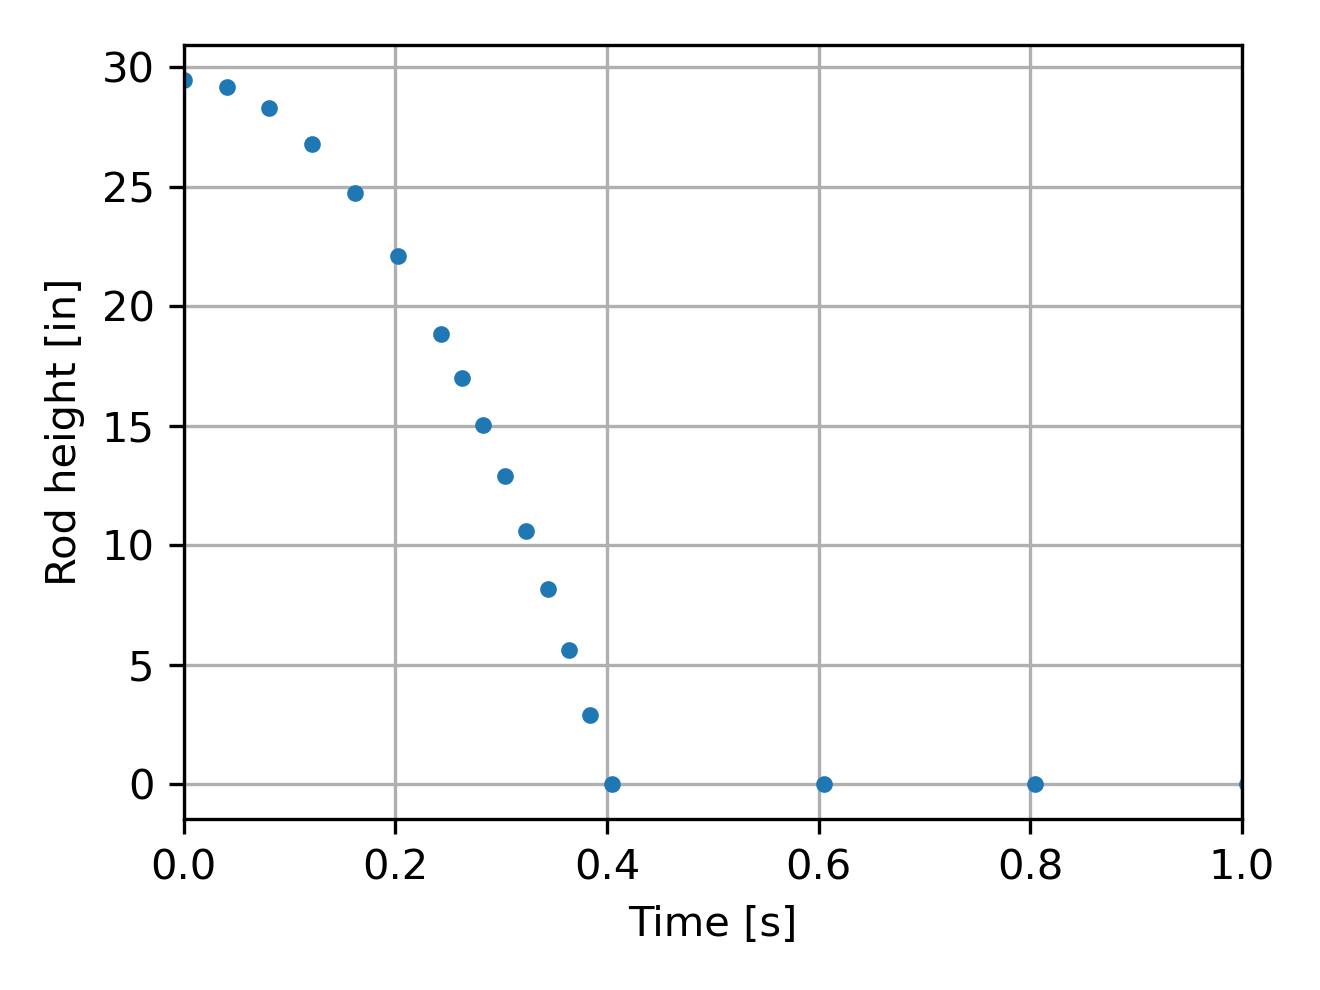
\includegraphics[width=0.7\columnwidth]{rod-height}
    \caption{Evolution of rod height evaluated at each timestep within the first second of the rod
    drop simulation. The rod reaches its fully inserted height at $t=0.4046$ s.}
    \label{fig:rod-height}
  \end{figure}
\end{frame}

\begin{frame}
  \frametitle{MSRE Rod Drop Experiment}
  \textbf{Nested Coupling Iteration Structure for the Rod Drop Simulation}
  \begin{figure}[t]
    \tikzstyle{every node}=[font=\small]
    \centering
    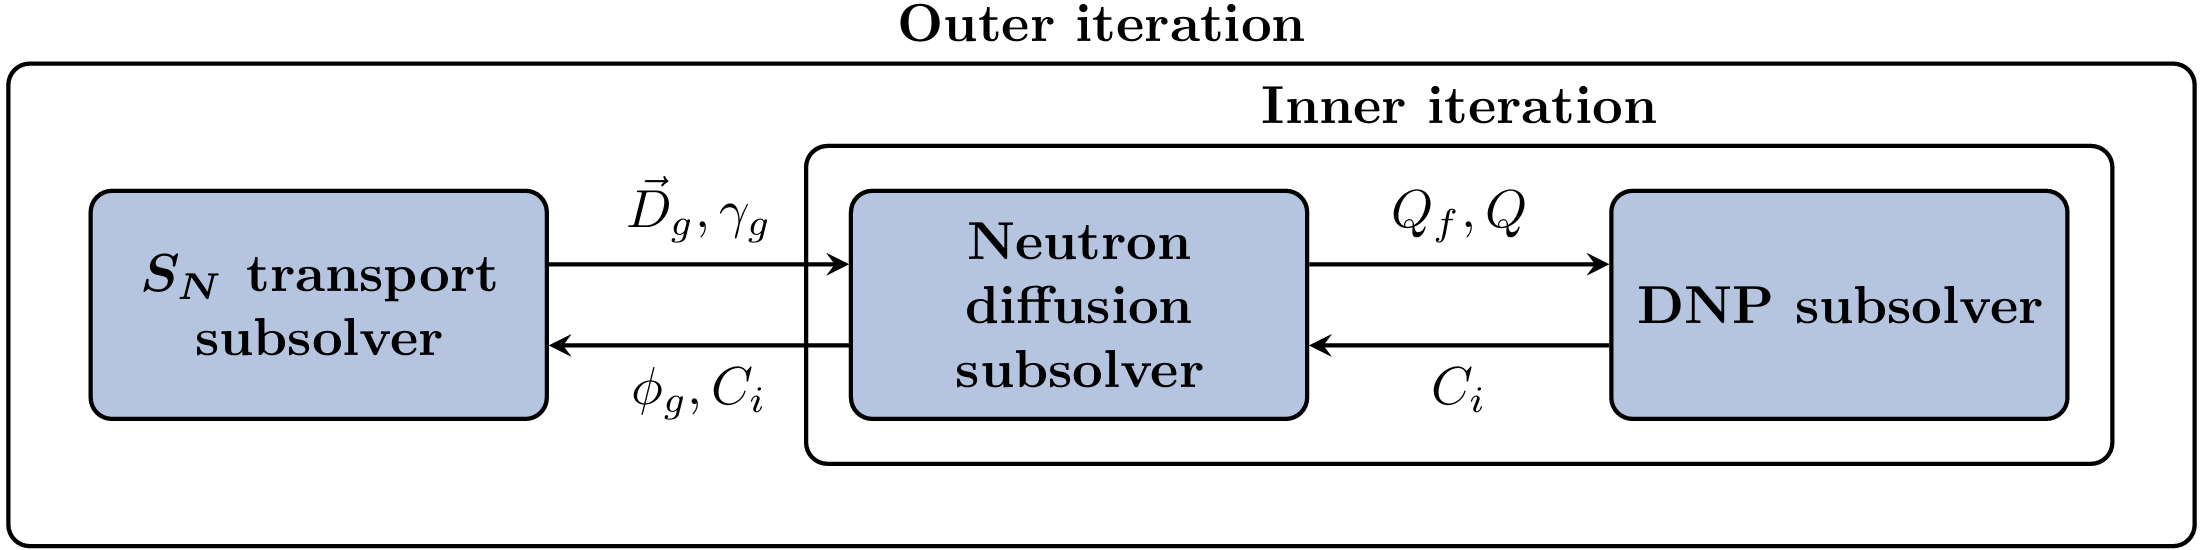
\includegraphics[width=\columnwidth]{images/nest-1}
    \caption{The nested iteration structure coupling the $S_N$, neutron diffusion, and \gls{DNP}
    solvers for the rod drop simulation using the hybrid $S_N$-diffusion method.}
    \label{fig:rod-drop-coupling}
  \end{figure}
\end{frame}

\begin{frame}
  \frametitle{MSRE Rod Drop Experiment}
  \textbf{Neutron Count Rate Following Rod Drop}
  \begin{columns}
    \column{5.5cm}
    \begin{figure}[t]
      \centering
      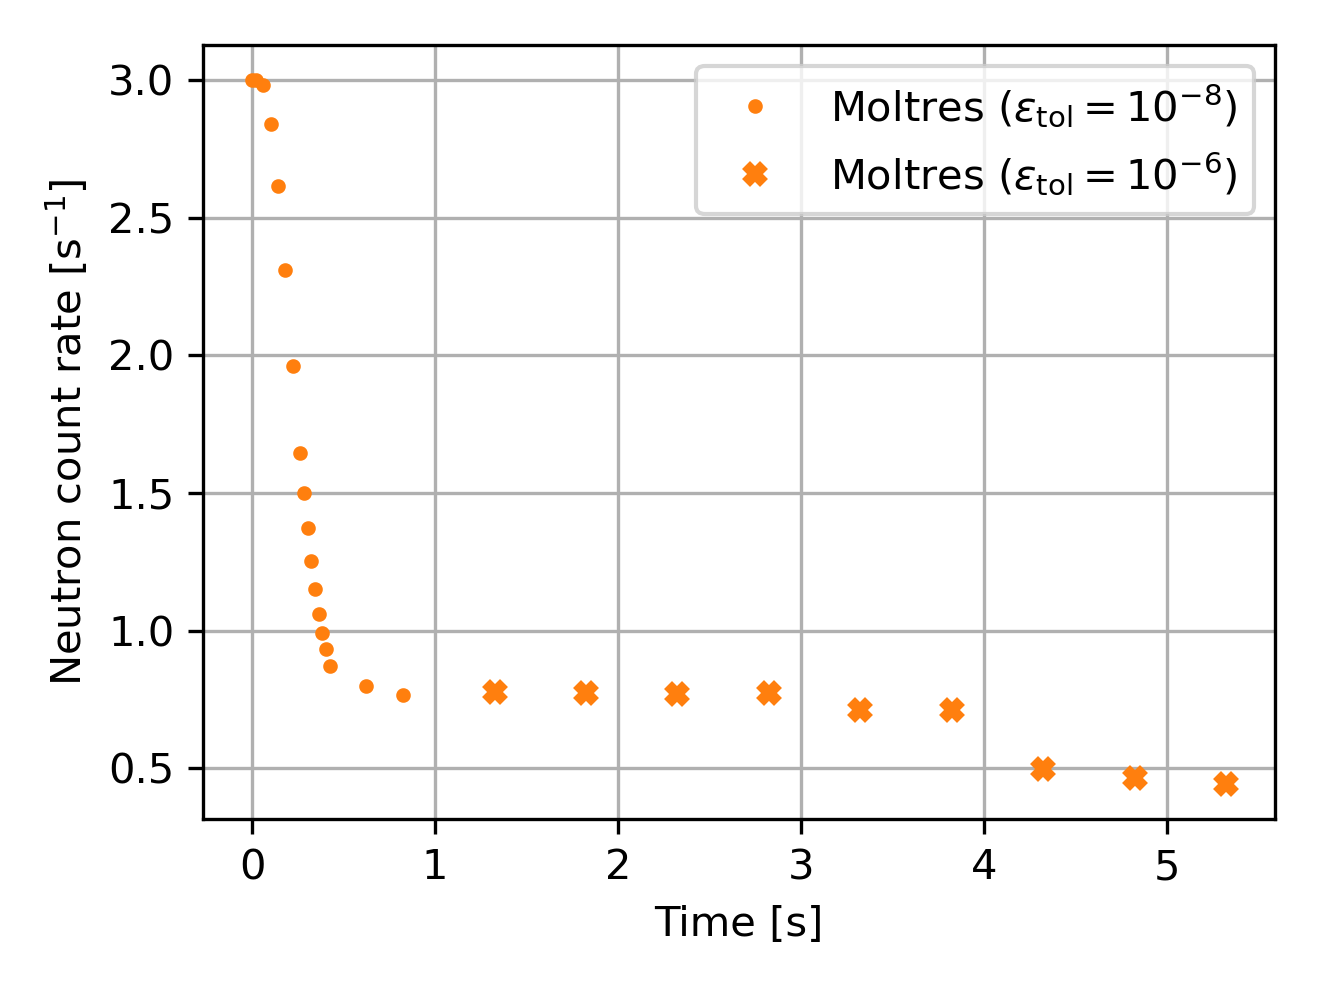
\includegraphics[width=\columnwidth]{count-rate}
      \caption{Neutron count rate during the rod drop experiment from Moltres rod drop simulation.}
      \label{fig:count-rate}
    \end{figure}
    \column{5.5cm}
    \begin{itemize}
      \item Steep initial decline in neutron count rate as the rod drops
      \item Decline in neutron count rate slows at $t=0.5$ s due to presence of DNPs
      \item Convergence issues prevented the simulation from converging from $t = 0.8$ s
      \item I raised the convergence tolerance to help the simulation continue
    \end{itemize}
  \end{columns}
%  \begin{itemize}
%    \item Moltres underpredicted the integral neutron count rate by approximately 20 \%.
%    \item Potential sources of error
%    \begin{itemize}
%      \item Uncertainty in the initial neutron count rate
%      \item Miscalculation of -1500 pcm reactivity withdrawal
%    \end{itemize}
%  \end{itemize}
\end{frame}

\begin{frame}
  \frametitle{MSRE Rod Drop Experiment}
  \textbf{Integral Neutron Count Following Rod Drop}
  \begin{columns}
    \column{5.5cm}
    \begin{figure}[t]
      \centering
      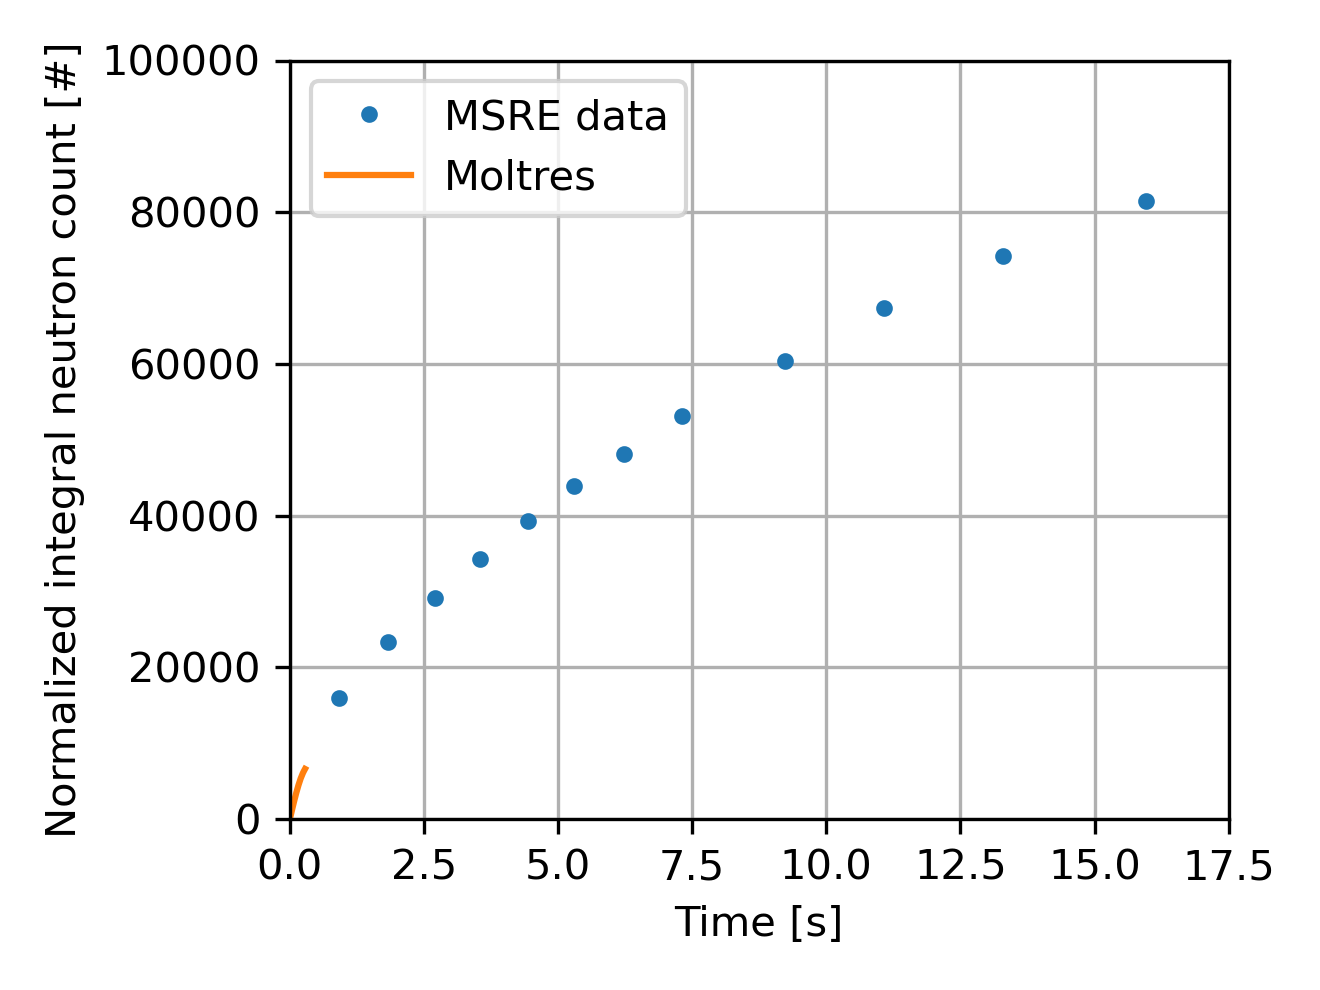
\includegraphics[width=\columnwidth]{integral-count}
      \caption{Integral neutron count during the rod drop experiment from \gls{MSRE} experimental data
      and hybrid method numerical results.}
      \label{fig:integral-count}
    \end{figure}
    \column{5.5cm}
    \begin{itemize}
      \item Moltres reproduces the expected trend in the integral neutron count rate
      \item Slight underprediction relative to MSRE rod drop experimental data
      \item Underprediction may be due to experimental uncertainty in $^{235}$U concentration,
        initial \& final rod height, initial neutron count rate.
    \end{itemize}
  \end{columns}
%  \begin{itemize}
%    \item Moltres underpredicted the integral neutron count rate by approximately 20 \%.
%    \item Potential sources of error
%    \begin{itemize}
%      \item Uncertainty in the initial neutron count rate
%      \item Miscalculation of -1500 pcm reactivity withdrawal
%    \end{itemize}
%  \end{itemize}
\end{frame}

%\begin{frame}
%  \frametitle{MSRE Reactivity Insertion Experiment}
%  \textbf{Nested Coupling Iteration Structure for the Reactivity Insertion Simulation}
%  \begin{figure}[t]
%    \centering
%    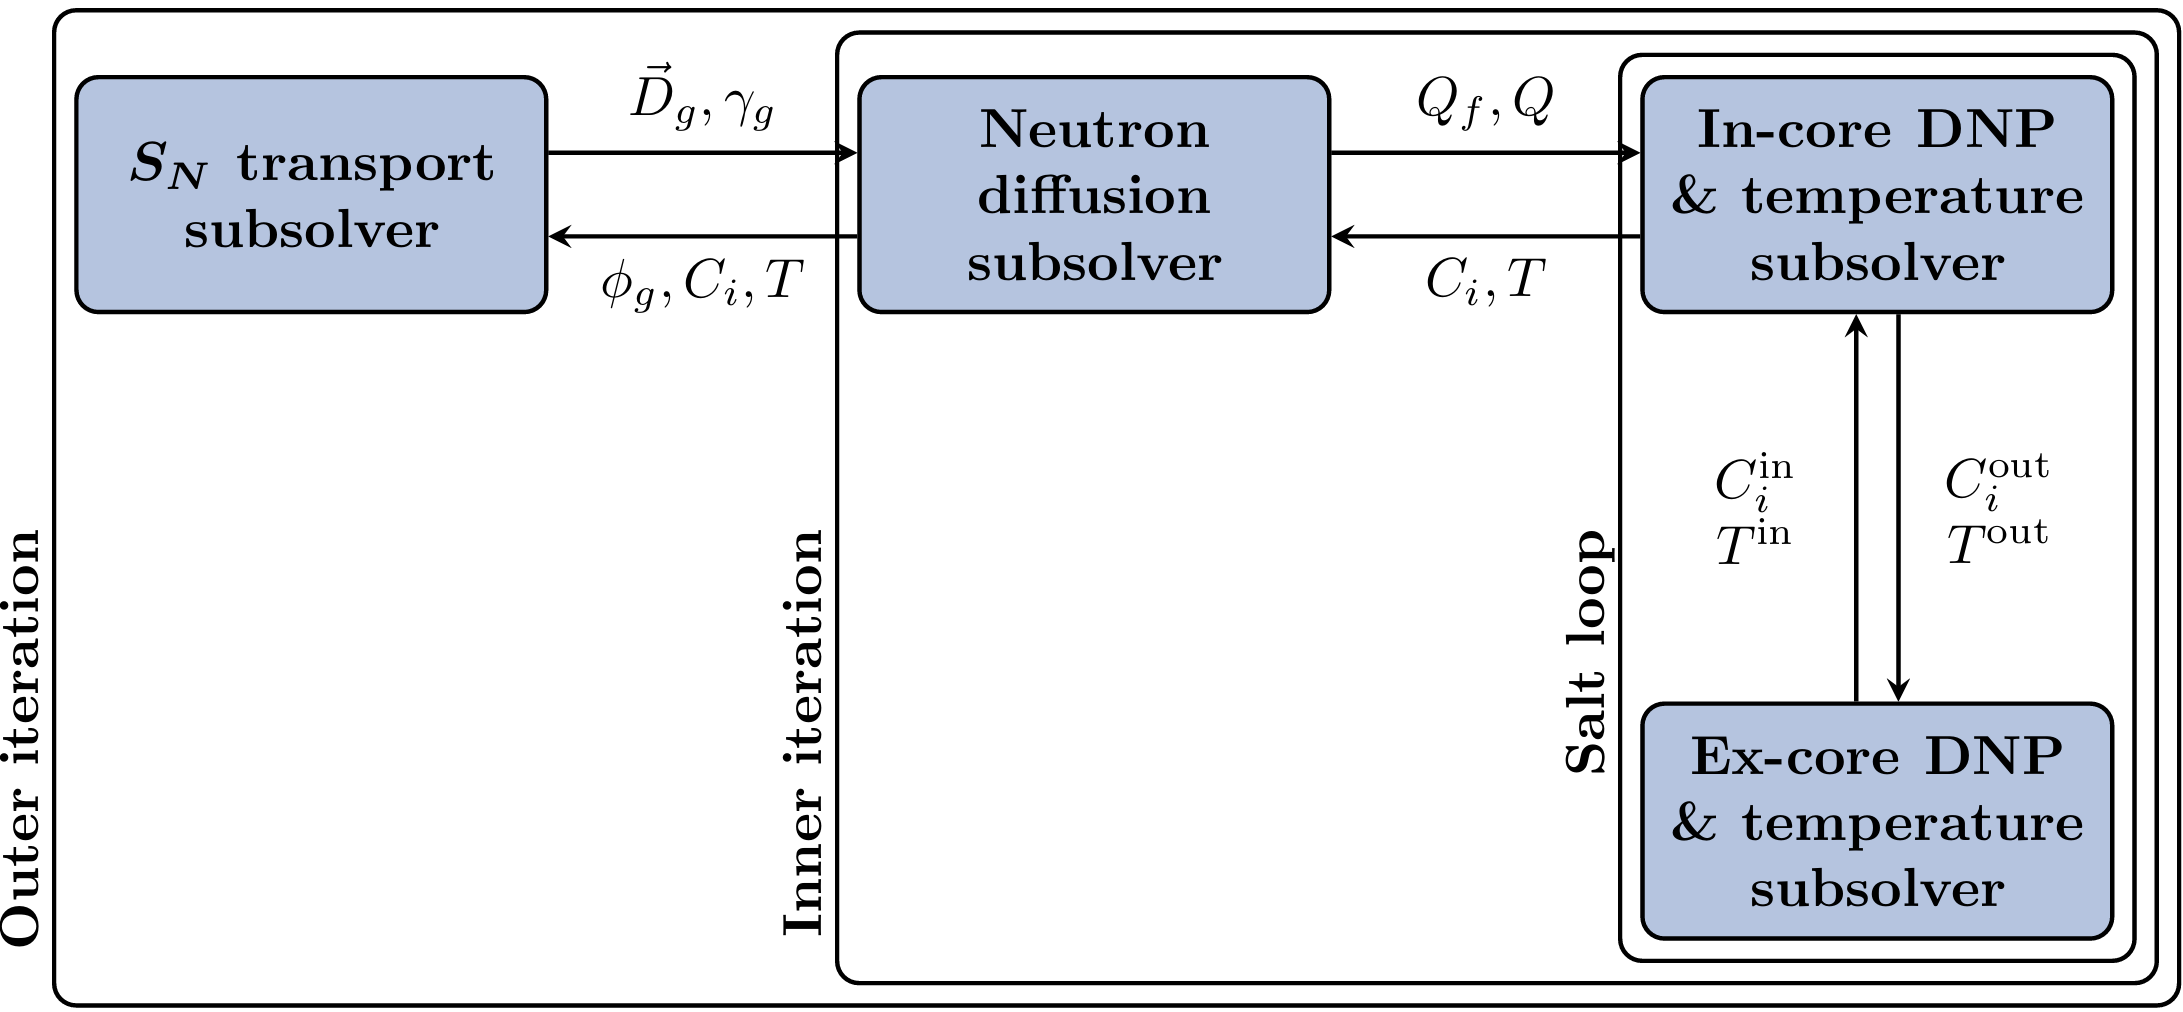
\includegraphics[width=\columnwidth]{images/nest-2}
%    \caption{The nested iteration structure coupling the $S_N$, neutron diffusion,
%    in-core \gls{DNP}-temperature, and ex-core
%    solvers for the reactivity insertion simulation using the hybrid $S_N$-diffusion method.}
%    \label{fig:insertion-coupling}
%  \end{figure}
%\end{frame}

\begin{frame}
  \frametitle{3-D Modeling with the Hybrid Method}
  \begin{block}{\textbf{Difficulties Faced During 3-D Modeling}}
  \begin{itemize}
    \item Poor convergence rate relative to 1-D \& 2-D modeling
    \begin{itemize}
      \item Likely due to increased streaming effects in 3-D near-void (air) regions in the reactor
    \end{itemize}
    \item Significant memory requirements
    \item Lagged control rod positions in fixed point iterations affecting convergence in time-dependent
      simulations $\Rightarrow$ simulation requires smaller timestep sizes
  \end{itemize}
\end{block}
\end{frame}
